\documentclass[a4paper,10pt]{article}
\usepackage[polish]{babel}
\usepackage[utf8]{inputenc}
\usepackage{polski}
\usepackage[T1]{fontenc}
\usepackage{enumerate}
\usepackage{indentfirst}
\usepackage{graphicx}
\usepackage{fancyhdr}
\usepackage{minted}
\usepackage[pdftex,pagebackref=false,draft=false,pdfpagelabels=false,
colorlinks=true,urlcolor=blue,linkcolor=red,citecolor=green,pdfstartview=FitH,
pdfstartpage=1,pdfpagemode=UseOutlines,bookmarks=true,bookmarksopen=true]{hyperref}


\setlength{\textheight}{24cm}
\setlength{\textwidth}{15.92cm}
\setlength{\footskip}{10mm}
\setlength{\oddsidemargin}{0mm}
\setlength{\evensidemargin}{0mm}
\setlength{\topmargin}{0mm}
\setlength{\headsep}{5mm}

\definecolor{code}{rgb}{0.95,0.95,1}

\renewenvironment{description}[1][0pt]
	{\list{}{\labelwidth=0pt \leftmargin=#1
	\let\makelabel\descriptionlabel}}
	{\endlist}

\author{Mateusz Gałażyn, Jeremi Niedziela}
\title{Krótki kurs tworzenia stron w technologii PHP}


\frenchspacing
\begin{document}

\pagestyle{fancy}
\lhead{Krótki kurs tworzenia stron w technologii PHP}


\maketitle
\section{Wstęp}
Ten krótki kurs ma na celu przedstawienie sposobu pisania stron przy użyciu technologii Apache + MySQL + PHP (w skrócie AMP) - jednego z najpopularniejszych zestawów oprogramowania służącego do uruchamiania serwisów WWW. Ten kurs jest bardzo okrojony i zawiera tylko wybrane elementy języka PHP oraz MySQL dlatego aby w pełni zrozumieć metodykę tworzenia aplikacji w oparciu o te  języki dobrze jest się wspierać dokumentacjami technicznymi, innymi kursami dostępnymi w internecie, a także specjalistycznymi forami dyskusyjnymi. \\
Dokumentacja PHP: \href{http://www.php.net/manual/pl/}{http://www.php.net/manual/pl/} \\
Dokumentacja MySQL: \href{http://dev.mysql.com/doc/refman/5.5/en/index.html}{http://dev.mysql.com/doc/refman/5.5/en/index.html} \\
Dokumentacja Apache: \href{http://httpd.apache.org/docs/2.4/}{http://httpd.apache.org/docs/2.4/} \\
Kurs PHP @ Wikibooks: \href{http://pl.wikibooks.org/wiki/PHP}{http://pl.wikibooks.org/wiki/PHP}

\subsection{Mechanizm działania systemu AMP} 
Gdy użytkownik strony uruchamia przeglądarkę i wpisuje w pasek adresu, adres szukanego serwisu WWW, przeglądarka nawiązuje połączenie z serwerem na którym są uruchomione usługi umożliwiające dostęp do strony. \\
\textbf{Apache} - jest to najszerzej stosowany w internecie serwer HTTP \\
\textbf{PHP} - jeden z najpopularniejszych języków programowania używany do tworzenia stron WWW. \\
\textbf{MySQL} - system zarządzania bazami danych za pomocą języka SQL \\


\begin{figure}[htbp]
\centering
\includegraphics[width=0.7\textwidth]{LAMP.png}
\caption{Schemat komunikacji zestawu AMP}
\end{figure}

Żądanie otrzymane od przeglądarki jest przechwytywane przez serwer Apache, który przetwarzając je uruchamia kod strony napisany w języku PHP. Następnie silnik PHP  komunikuje się z bazą danych, pobiera dane, przetwarza je i zamienia na kod HTML, który zwraca serwerowi Apache. W kolejnym kroku serwer Apache wysyła kod HTML razem z obrazami umieszczonymi na stronie i stylami do przeglądarki, która renderuje i wyświetla stronę.

\section{Instalacja środowiska AMP}
\subsection{Instalacja na systemie Windows}
\subsubsection{Instalacja serwera Apache}
\subsubsection{Instalacja PHP}
\subsubsection{Instalacja serwera MySQL}
\subsection{Instalacja na systemie Linux}
\subsubsection{Instalacja serwera Apache}
\subsubsection{Instalacja PHP}
\subsubsection{Instalacja serwera MySQL}
\subsection{Konfiguracja}
\subsubsection{Konfiguracja Apache}
%TODO stworzenie katalogu na forum
%TODO stworzenie katalogu na PMA
\subsubsection{Konfiguracja PHP}
%TODO konfiguracja timezone
%TODO ustawienie error_level i notice
%TODO włączenie rozszerzeń PDO, etc...
\subsubsection{Konfiguracja MySQL}
% ustawianie hasła roota
\subsection{Instalacja phpMyAdmin}
% opis instalacji jak i interfejsu
\section{Projekt forum dyskusyjnego}
Naszym celem jest jest zbudowanie prostego forum dyskusyjnego. Musimy dać możliwość rejestrowania się poszczególnym użytkownikom, dodawania własnych wątków oraz odpowiadania na już utworzone. Potrzebne będzie też konto administratora, który będzie miał prawo moderacji odpowiedzi w tematach (postów).
\subsection{Układ podstron}
Gdy zostanie już ustalona lista wymaganych funkcjonalności projektowanego serwisu, następnym etapem jest stworzenie układu poszczególnych podstron.
\paragraph{Strona główna} Tutaj trzeba wyświetlić listę tematów (wraz z odnośnikami do podstrony, na którym będzie pojedynczy wątek wyświetlany w całości) które zostały założone na forum, umieścić odnośniki do podstrony z formularzem używanym do zalogowania się i rejestracji dla użytkowników oraz odnośnik do podstrony umożliwiającej założenie nowego tematu.
\paragraph{Podstrona wątku} W tym miejscu trzeba wyświetlić wszystkie posty w danym wątku, oraz formularz dający możliwość odpowiedzi w tym wątku. Gdy administrator wejdzie na tą podstronę, trzeba dać także dodatkowe możliwości edycji i usuwania poszczególnych postów.
\paragraph{Podstrona logowania} Zawierać będzie formularz logowania umożliwiający uwierzytelnienie użytkownika wchodzącego stronę. Uwierzytelnienie będzie polegało na porównaniu nazwy użytkownika i hasła z obecnymi w bazie danych. Po zalogowaniu się, użytkownik zostanie przekierowany z powrotem na stronę główną. Podstrona dostępna tylko dla niezalogowanych użytkowników.
\paragraph{Podstrona rejestracji} Odpowiedzialna za obsługę rejestracji nowego użytkownika. Trzeba będzie wyświetlić formularz rejestracji, odebrać i zweryfikować dane oraz dodać je do bazy danych.

\paragraph{Podstrona nowego wątku} Podstrona z formularzem umożliwiającym dodanie nowego wątku. Po odebraniu danych od użytkownika trzeba będzie dokonać ich weryfikacji i dodać do bazy danych. Na koniec trzeba przekierować użytkownika do podstrony wątku.

\paragraph{Podstrona edycji postu} Podstrona z formularzem umożliwiającym edycję własnych postów, a także w przypadku administratora - edycji każdego postu. Przekierowuje z powrotem do podstrony wyświetlającej cały wątek. \\

\begin{figure}[htbp]
\centering
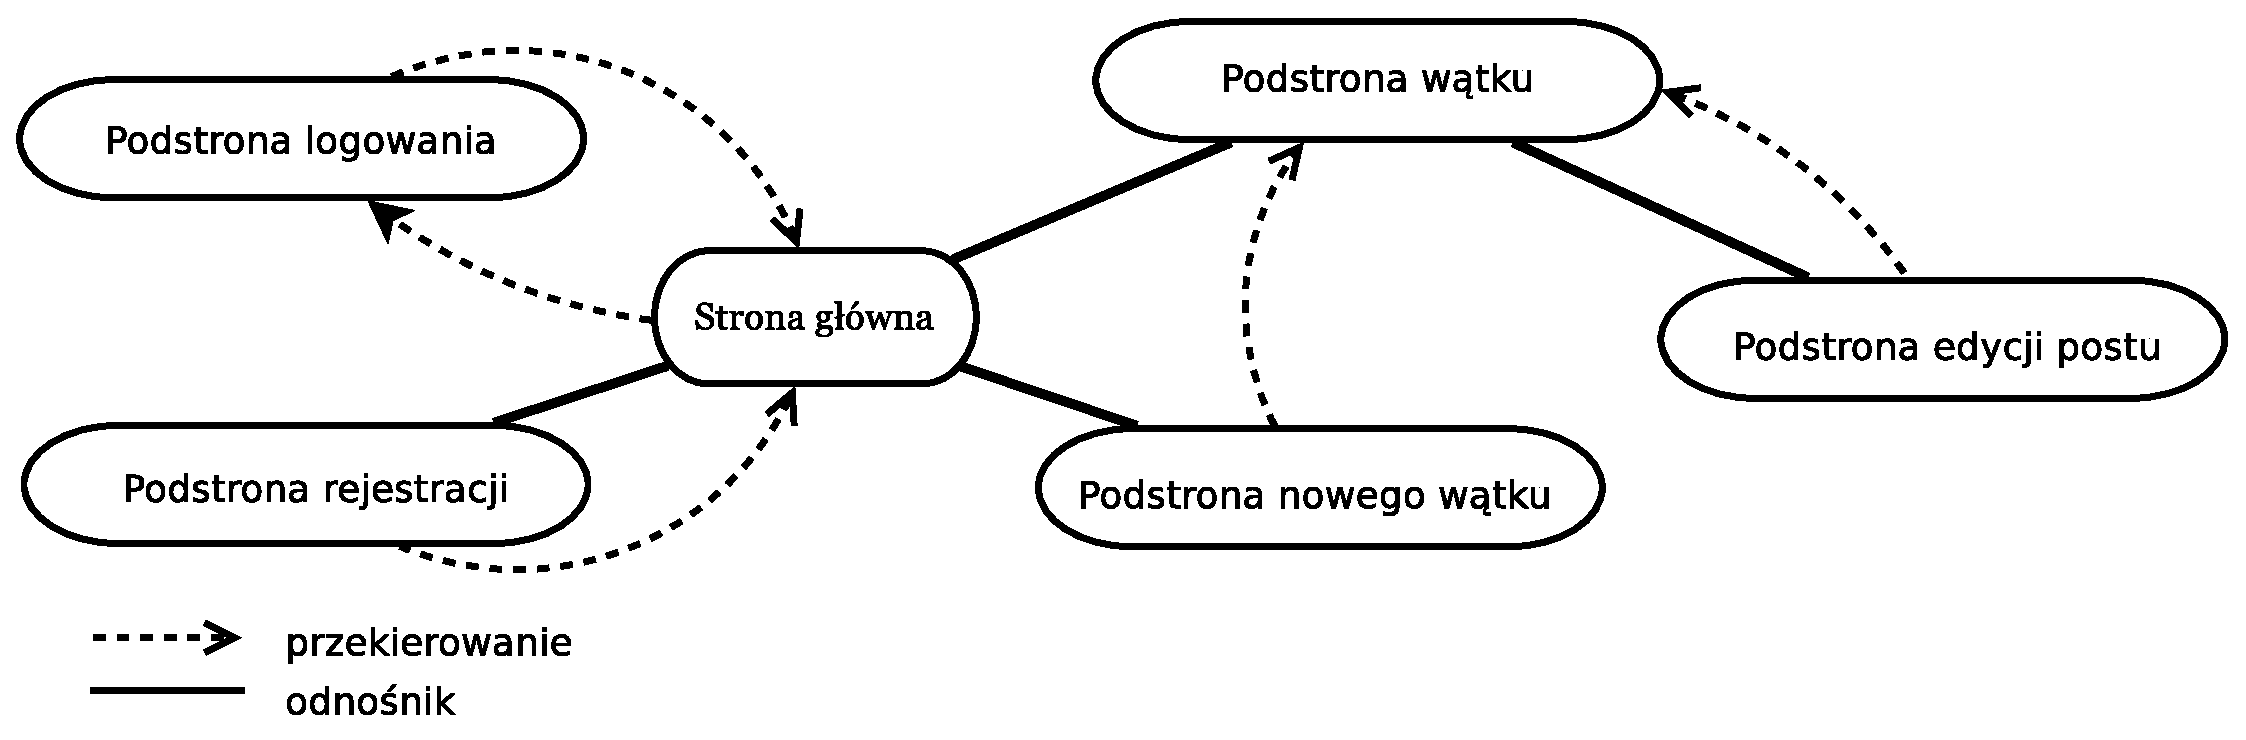
\includegraphics[width=0.9\textwidth]{subp.eps}
\caption{Układ podstron forum}
\end{figure}


\subsection{Projekt bazy danych}
Informacje w bazie danych są przechowywane w postaci tabel, podobnie jak w arkuszach kalkulacyjnych dostępnych w popularnych pakietach biurowych. W bazie projektowanego forum będziemy przechowywać listę użytkowników, listę tematów oraz listę postów. Dla każdej z tych list trzeba utworzyć oddzielną tabelę: users, threads, posts. W każdej z tych tabel konieczne jest stworzenie odpowiednich kolumn służących do przechowywania danych we właściwych typach. Ustawienie typu danej przechowywanej w każdej kolumnie przyśpiesza pracę serwera MySQL poprzez automatyczną optymalizację realizowanych zapytań do bazy oraz optymalizację sposobu przechowywania tabel na dysku.
\subsubsection{Typy danych MySQL}
W języku MySQL jest wiele typów danych 
(dokładny opis: \href{http://dev.mysql.com/doc/refman/5.5/en/data-type-overview.html}{http://dev.mysql.com/doc/refman/5.5/en/data-type-overview.html}), te najważniejsze to:

\paragraph{Typy znakowe:}
\begin{description}[5mm]
\item[CHAR] Przechowuje ciąg znaków do 255 elementów.
\item[VARCHAR] Tak jak \textbf{CHAR} przechowuje ciąg znaków do 255 elementów. Główną różnicą pomiędzy nimi jest to, że \textbf{VARCHAR} zmienia swój rozmiar w zależności od przyjętej liczby znaków, a \textbf{CHAR} zawsze rezerwuje miejsce 255 znaków niezależnie od długości zapisywanego ciągu.
\item[TEXT] Przechowuje ciąg do 65535 znaków.
\item[MEDIUMTEXT] Przechowuje ciąg do 16777215 znaków.
\end{description}

\paragraph{Typy liczbowe:}
\begin{description}[5mm]
\item[TINYINY] Przechowuje liczby od -128 do 127 (0 do 255 w przypadku \textbf{UNSIGNED}).
\item[SMALLINT] Przechowuje liczby od -32768 to 32767 (0 do 65535 w przypadku \textbf{UNSIGNED}).
\item[MEDIUMINT] Przechowuje liczby od -8388608 do 8388607 (0 do 16777215 w przypadku \textbf{UNSIGNED}).
\item[FLOAT] Małe liczby zmiennoprzecinkowe.
\item[DOUBLE] Liczby zmiennoprzecinkowe o podwojonej precyzji.
\end{description}
Każdy typ liczbowy występuje także w wersji \textbf{UNSIGNED}, która pozwala przechowywać dwa razy większe liczby bez przechowywania informacji o znaku.
\paragraph{Inne typy:}
\begin{description}[5mm]
\item[DATE] Data w formacie YYYY-MM-DD
\item[DATETIME] Data w formacie YYYY-MM-DD HH:MM:SS
\item[TIMESTAMP] Znacznik czasu w formacie: YYYYMMDDHHMMSS
\item[TIME] Czas w formacie: HH:MM:SS
\item[ENUM] Podobnie jak w C++, definiuje listę określonych wartości jakie może przyjąć to pole.
\item[SET] Podobnie jak \textbf{ENUM}, lecz pole w tabeli może przyjąć kilka wartości na raz.
\end{description}

\subsubsection{Projekty tabel}
Tabela \textit{users} powinna zawierać kolumny przechowujące informacje o użytkowniku takie jak: nazwa użytkownika, login używany przy identyfikacji na stronie, hash SHA-1\footnote{W bazach danych \textbf{NIGDY} nie powinno się przechowywać haseł w jawnej postaci tekstu. W przypadku gdy osoba trzecia uzyska nieautoryzowany dostęp do bazy danych, będzie mogła skopiować listę haseł wszystkich użytkowników, co nie powinno mieć nigdy miejsca. Zamiast tego przechowuje się specjalne hashe wygenerowane na podstawie haseł. Więcej informacji na temat hashy: \href{http://pl.wikipedia.org/wiki/Funkcja_skrótu}{pl.wikipedia.org}} hasła oraz pole determinujące czy dany użytkownik ma uprawnienia administracyjne (wartość 1, gdy użytkownik jest administratorem). \\
Tabela \textit{threads} powinna zawierać kolumny przechowujące tytuł wątku, zawartość pierwszego posta oraz data utworzenia wątku. \\
Tabela \textit{posts} powinna zawierać kolumny przechowujące treść posta i datę jego utworzenia. \\
Dodatkowo w każdej z tabel powinna znajdować się kolumna \textit{id} identyfikująca w każdej tabeli pojedynczy rekord. To rozwiązania ułatwia odwoływanie się do poszczególnych wpisów (rekordów)  w tabeli, bez konieczności ponownego przeszukiwania całej tabeli.
W tabelach \textit{posts} i  \textit{threads} oprócz informacji o postach i wątkach musimy utworzyć tak zwane relacje - kolumny wiążące poszczególne posty z użytkownikami oraz wątkami. Jest to tak zwana relacja \textbf{jeden do wielu}. Zagadnienie to można rozwiązać w prosty sposób: w tabeli \textit{threads} tworzymy kolumnę \textit{author\_id}, którą będzie zawierała id rekordu w tabeli \textit{users} odpowiadającego użytkownikowi, który stworzył dany wątek. Analogiczną operację trzeba wykonać dla tabeli posts: tworzymy kolumnę \textit{author\_id} oraz dodatkową \textit{thread\_id}, która definiuje wątek do którego przynależy dany post.

\begin{figure}[htbp]
\centering
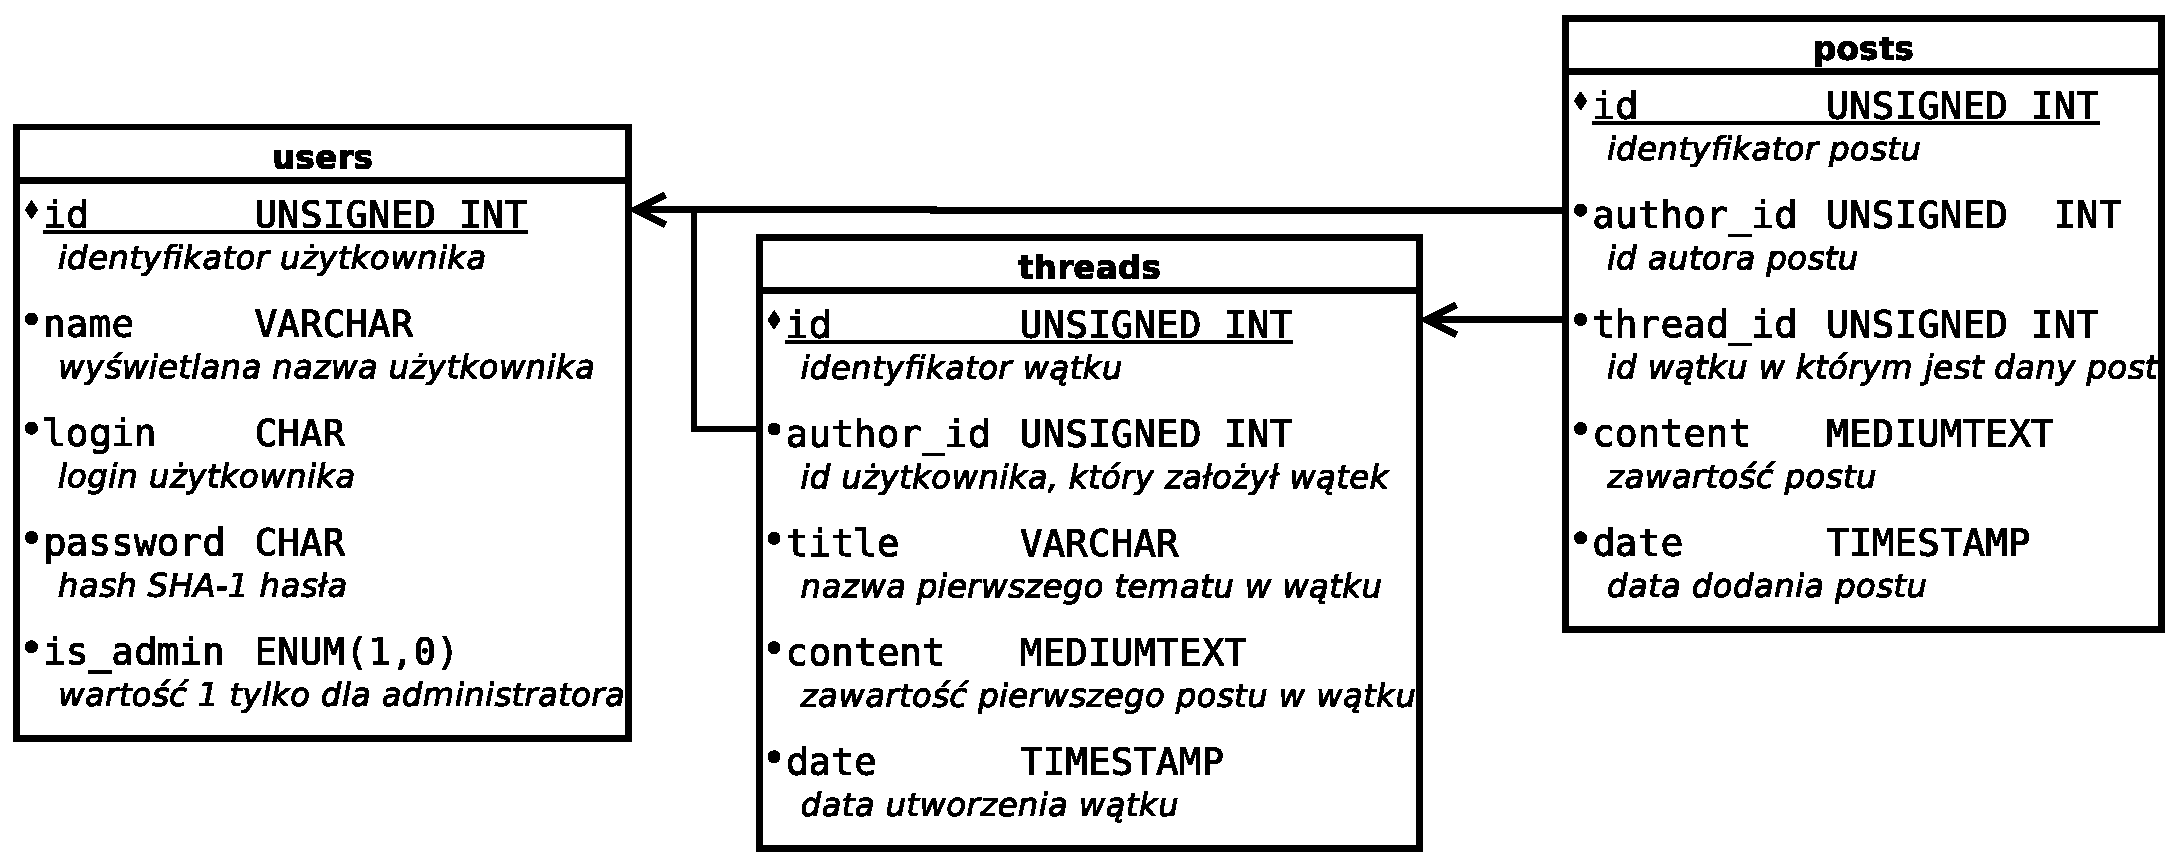
\includegraphics[width=1\textwidth]{db.eps}
\caption{Schematy tabel i ich wzajemne relacje}
\end{figure}

\paragraph{Optymalizacja}
Oprócz precyzowania typów danych dla każdej kolumny, aby ułatwić sobie i serwerowi pracę można zdefiniować dodatkowe atrybuty dla poszczególnych kolumn. Kolumna \textit{id} występująca w każdej z tabel musi być zdefiniowana z atrybutami \textit{PRIMARY KEY} (co jest zaznaczone na schemacie podkreśleniem) - oznacza to, że kolumna jest wykorzystywana do identyfikacji rekordów w tabeli, \textit{AUTO\_INCREMENT} - każdy dodawany rekord ma ustawiane automatycznie \textit{id} o 1 większe niż największe \textit{id} w tabeli, \textit{NOT NULL} - nie może mieć wartości 0.

\subsubsection{Kod SQL}
Nadszedł czas na stworzenie zaprojektowanej przez nas struktury tabel. Uruchamiamy serwer MySQL, a następnie poleceniem (dla systemu Linux): \\
\begin{minted}[bgcolor=code]{bash}
mysql -u root -p
\end{minted}
uruchamiamy wiersz poleceń MySQL.
Na systemie Windows aby uruchomić wiersz poleceń, wpierw trzeba uruchomić terminal, a w nim wpisać:  \\
\begin{minted}[bgcolor=code]{bat}
C:> cd C:\sciezka\do\katalogu\mysql\bin
C:\sciezka\do\katalogu\mysql\bin> mysql.exe -u root -p
\end{minted}
Następnie po wpisaniu hasła, aby stworzyć bazę danych wydajemy polecenie: \\
\begin{minted}[bgcolor=code]{sql}
CREATE DATABASE forum;
\end{minted}
Aby przystąpić do tworzenia tabel, trzeba wybrać nowo utworzoną bazę danych: \\
\begin{minted}[bgcolor=code]{sql}
USE forum;
\end{minted}
Możemy teraz utworzyć tabelę \textit{users} wydając poniższe polecenie: \\
\begin{minted}[linenos=true, bgcolor=code]{sql}
CREATE TABLE `forum`.`users` (
	`id` INT UNSIGNED NOT NULL AUTO_INCREMENT PRIMARY KEY ,
	`name` VARCHAR( 255 ) NOT NULL ,
	`login` CHAR( 255 ) NOT NULL ,
	`password` CHAR( 255 ) NOT NULL ,
	`is_admin` ENUM( '1', '0' ) NOT NULL ,
	UNIQUE (
		`name` ,
		`login` 
	)
);
\end{minted}
Ważne jest umieszczenie na końcu wyrażenia średnika, ponieważ informuje to interpreter MySQL że to jest koniec komendy. Bez średnika interpreter będzie czekał na dalsze wprowadzanie komend, dopóki nie napotka średnika.
W linii 1 podajemy nazwę bazy danych, a po kropce jest nazwa tworzonej tabeli. Nazwy bazy, tabel i kolumn są wzięte w ` `. W liniach 2-6 zdefiniowane są kolumny tabeli oddzielone przecinkami. Składnia jest następująca: \\
\begin{minted}[bgcolor=code]{sql}
`nazwa_kolumny` TYP NULL [dodatkowe atrybuty] ,
\end{minted}
Na początku podajemy nazwę kolumny, potem nazwę typu, jeżeli jest to typ liczbowy bez znaku, za nazwą typu dodajemy \textit{UNSIGNED}. Jeżeli jest to typ znakowy \textit{CHAR} lub \textit{VARCHAR} to wpisujemy w nawiasie maksymalną długość ciągu znaków. Jeżeli jest to typ \textit{ENUM}, lub \textit{SET} w nawiasie podajemy dopuszczalne wartości. Następnie podajemy informację czy w tą kolumnę może zostać wpisana wartość pusta - parametr \textit{NULL}, lub gdy nie: \textit{NOT NULL}. Jeżeli chcemy ustawić dodatkowe opcje dla kolumny wpisujemy je oddzielając spacją. Dla kolumny \textit{id} zostały ustawione opcje \textit{AUTO\_INCREMENT} oraz \textit{PRIMARY KEY}. Po wymienionych kolumnach można zdefiniować dodatkowe indeksy, w linii 7 zdefiniowany jest indeks \textit{UNIQUE}: dla kolumn umieszczonych w nawiasie wartości w pól w rekordach nie mogą się powtarzać. \\
Tabela \textit{threads}: \\
\begin{minted}[linenos=true, bgcolor=code]{sql}
CREATE TABLE `forum`.`threads` (
	`id` INT UNSIGNED NOT NULL AUTO_INCREMENT PRIMARY KEY ,
	`author_id` INT UNSIGNED NOT NULL ,
	`title` VARCHAR( 255 ) NOT NULL ,
	`content` MEDIUMTEXT NOT NULL ,
	`date` TIMESTAMP ON UPDATE CURRENT_TIMESTAMP NOT NULL DEFAULT CURRENT_TIMESTAMP 
);
\end{minted}
Kod jest prawie identyczny jak w poprzednim przypadku. Różnica pojawia się jedynie w linii 6. Po typie danych \textit{TIMESTAMP} zdefiniowana jest opcja \textit{ON UPDATE CURRENT\_TIMESTAMP}, która mówi, że po aktualizacji rekordu silnik bazy danych automatycznie umieści w kolumnie \textit{date} aktualny znacznik czasu. Następnie jest podana informacja, że wartość pola nie może być wartością \textit{NULL}. Parametr \textit{DEFAULT CURRENT\_TIMESTAMP} mówi nam, że gdy przy wpisywaniu wartości do bazy danych nie podamy wartości tego pola, serwer MySQL automatycznie wypełni to pole aktualną godziną. \\
Tabela \textit{posts}: \\
\begin{minted}[linenos=true, bgcolor=code]{sql}
CREATE TABLE `forum`.`posts` (
`id` INT UNSIGNED NOT NULL AUTO_INCREMENT PRIMARY KEY ,
`author_id` INT UNSIGNED NOT NULL ,
`thread_id` INT UNSIGNED NOT NULL ,
`content` MEDIUMTEXT NOT NULL ,
`date` TIMESTAMP ON UPDATE CURRENT_TIMESTAMP NOT NULL DEFAULT CURRENT_TIMESTAMP 
);
\end{minted}
Składnia jest analogiczna jak w poprzednim wypadku. Powyższe trzy zapytania \textit{CREATE} tworzą już kompletną, ale jeszcze pustą strukturę naszej bazy danych.
\section{Kod strony}
Przed przystąpieniem do pracy nad kodem strony, warto wyposażyć się w jakikolwiek edytor z kolorowaniem składni. Na systemy z rodziny Windows dobrym rozwiązaniem jest Notepad++, dostępny ze strony: \href{http://notepad-plus-plus.org/download/v6.1.2.html}{http://notepad-plus-plus.org/download/v6.1.2.html}. Na systemach GNU (w tym tych z rodziny Linux) może to być Emacs, Vim, Nano lub używany w środowisku Gnome, Gedit.
\subsection{Składnia języka PHP}
Przykładowy kod strony w języku php: \\
\begin{minted}[linenos=true, bgcolor=code]{php}
<?php
$jeden = 'bar';
$dwa = "foo";
$trzy = null;
$liczba = "4";
$liczba2 = 3;
if($liczba % 2 == 0)
{
	echo 'liczba jest podzielna przez 2 <br />';
}
else
{
	echo 'liczba nie jest podzielna przez 2 <br />';
}

if($liczba == 4)
	echo 'Ta liczba to 4!';
elseif($liczba < 4)
	echo 'Ta liczba jest mniejsza od 4.<br />';
else
	echo 'Ta liczba jest wieksza od 4 <br />';
echo $jeden.$dwa.($liczba+$liczba2);
?>
\end{minted}
Zapisując powyższy kod jako plik \textit{index.php} w katalogu \textit{DocumentRoot} zdefiniowanym przy Konfiguracji Apache, a następnie wchodząc na stronę http://127.0.0.1/ otrzymamy wynik:
\begin{minted}{php}
liczba jest podzielna przez 2
Ta liczba to 4!
barfoo7
\end{minted}
Kod PHP aby został wykonany musi być zawarty w tagach \textit{<?php ?>}.
W linijkach 2 - 6 zostały zdefiniowane zmienne. Nazwy zmiennych muszą być poprzedzone znakiem \$ zarówno przy definiowaniu jak i późniejszym odwoływaniu się do nich. Ciąg znaków przypisywany do zmiennej można zawszeć w apostrofach lub cudzysłowach. Między tymi dwoma sposobami jest niewielka różnica: gdy zawrzemy ciąg znaków w cudzysłowach PHP przeszukuje zawartość ciągu pod kątem znaków specjalnych (np.: \textbackslash n \textbackslash r itp.), w przypadku apostrofów przeszukiwanie nie jest dokonywane (ta forma jest nieco szybsza). W liniach 7 - 21 są umieszczone struktury \textit{if - else}. W linii 7 jest wykonywane modulo na zmiennej \textit{\$liczba}, a następnie wynik tej operacji jest przyrównywany do zera. Należy zwrócić uwagę iż w PHP brak jest typów zmiennych - zależnie od potrzeb zmienna jest automatycznie traktowana jako ciąg znaków, lub jako liczba. W linii 9 do wyświetlania jest używana struktura języka: \textit{echo}. W linii 22 został użyty operator konkatenacji (kropka) do połączenia trzech ciągów znaków w jeden. Najpierw zostało wykonane dodawanie dwóch liczb w nawiasie, a następnie ich suma została zamieniona na ciąg znaków, który został doklejony do fraz 'bar' i 'foo'. W PHP operator kropki nie jest używany w odniesieniu do obiektów (jak to ma miejsce w Javie i w C++). \\
Przykładowa klasa w PHP: \\
\begin{minted}[linenos=true, bgcolor=code]{php}
<?php
class Telewizor
{
	private static $iloscTelewizorow = 0;
	
	private $aktualnyKanal = 0;
	private $poziomGlosnosci = 50;
	
	public static function pobierzLiczbeTelewizorow()
	{
		return self::$iloscTelewizorow;
	}
	
	public function __construct()
	{
		++self::$iloscTelewizorow;
	}
	
	public function ustawGlosnosc($poziomGlosnosci)
	{
		$this->poziomGlosnosci = $poziomGlosnosci;
	}
	
	public function ustawKanal($nrKanalu = 0)
	{
		$this->aktualnyKanal = $nrKanalu;
	}
};

function wyswietlaj()
{
	echo 'teraz wyswietlaja '.Telewizor::pobierzLiczbeTelewizorow().' telewizory';
}

new Telewizor;
new Telewizor;
$sharp =  new Telewizor;
$sharp->ustawKanal();
$sharp->ustawKanal(13);
$sharp->ustawGlosnosc(30);
$sharp->ustawGlosnosc(10);

wyswietlaj();
?>
\end{minted}
Wynik:
\begin{minted}{php}
teraz wyswietlaja 3 telewizory
\end{minted}
Składnia jest bardzo podobna do tej znanej z C++, za wyjątkiem braków typów zmiennych. W liniach 4 - 7 zostały zadeklarowane i zainicjalizowane domyślnymi wartościami właściwości klasy. W linii 11 jest odwołanie do statycznej właściwości klasy. W PHP dostęp do statycznych pól klasy jest uzyskiwany za pomocą wyrażenia self i operatora dostępu "::". W linii 14 znajduje się konstruktor, którego zadaniem jest zwiększanie ilości stworzonych telewizorów. W PHP konstruktory i destruktory noszą zawsze nazwę \textit{\_\_construct()} i \textit{\_\_destruct()} niezależnie od nazwy klasy. W deklaracji każdej funkcji i metody zawsze znajduje się słowo kluczowe function. W linii 21 jest ustawiany poziom głośności w telewizorze. Dostęp do właściwości obiektów uzyskać można tylko za pomocą wskaźnika \textit{\$this} wskazującego na aktualny obiekt, dostępnego w każdej \textbf{niestatycznej} metodzie klasy. Należy zwrócić uwagę, że gdy odwołujemy się do właściwości klasy za pomocą \textit{\$this} nie używamy już \textit{\$} przed nazwą pola klasy. W linii 24 została zdefiniowana funkcja przyjmująca parametr, który ma już wartość domyślną. Jest to pewien odpowiednik znanego z C++ przeciążania funkcji, gdy kilka funkcji mogło mieć tą samą nazwę - różnił je tylko zestaw argumentów. W PHP przeciążanie funkcji znane z C++ jest niedozwolone, zamiast tego stosuje się wartości domyślne argumentów. Pozwala to na wywołanie funkcji bez podawania argumentów, którym zostały przypisane wartości domyślne w nagłówku funkcji. Przykład takiego wywołania jest w linii 38 i 39.
Obiekty tworzy się za pomocą operatora \textit{new}, przykład znajduje się w liniach 35 - 37. W liniach 35 i 36 tworzone są obiekty klasy Telewizor, które nie są do niczego przypisywane. W linii 37 tworzony obiekt tej samej klasy przypisany do zmiennej \textit{\$sharp}. Dostęp do pól i metod uzyskiwany jest za pomocą operatora -> .
\paragraph{Zagnieżdżanie wewnątrz kodu HTML} PHP umożliwia przeplatanie kodu HTML i PHP, co umożliwia generowanie zawartości stron w czasie rzeczywistym. Przykład kodu: \\
\begin{minted}[linenos=true, bgcolor=code]{php}
<!DOCTYPE HTML>
<html>
<head>
 <title>Forum</title>
 <meta charset="UTF-8" />
</head>
<body>
<?php if(!is_object(User::$oCurrentUser)):?>
<a href="register.php">rejestracja</a>
<?php else: ?>
Witaj <b><?php echo User::$oCurrentUser->sName; ?></b>
<?php endif; ?>
<br /><br />
<?php if(count($aThreads) > 0):?>
Lista watkow na forum:
<table border="1">
<?php foreach($aThreads as $i => $oThread): ?>
<tr>
 <td><?php echo $i+1 ?></td>
 <td>
<a href="thread.php?id=<?php echo $oThread->iId ?>">
<?php echo $oThread->sTitle ?></a>
<?php 
 if(is_object(User::$oCurrentUser))
	 if(User::$oCurrentUser->bIsAdmin)
	 	echo ' <a href="delete.php?tid='.$oThread->iId.'">[ usun ]</a>'; 
?></td>
 <td><?php echo $oThread->sAuthorName ?></td>
 <td><?php echo $oThread->sDate ?></td>
</tr>
<?php endforeach?>
</table>
<?php else: ?>
Brak watkow na forum.
<?php endif;?>
</body>
</html>
\end{minted}
W linii 8 jest wstawiona funkcja \textit{if()}. Należy zwrócić uwagę na dwukropek postawiony za nawiasem - w tym wypadku cała zawartość aż do linii 10, w której występuje \textit{else:} jest wyświetlana gdy warunek jest spełniony\footnote{dokładnie: gdy statyczne pole klasy \textit{User::\$oCurrentUser} nie jest obiektem - służy do tego funkcja \textit{\href{http://www.php.net/manual/en/function.is-object.php}{is\_object()}}}. Koniec \textit{if()} jest w linii 12. W linii 11 wyświetlane jest pole \textit{sName} zmiennej \textit{User::\$oCurrentUser} za pomocą wyrażenia \textit{echo}. W linii 17 występuje wyrażenie \textit{foreach()}. Ten zapis należy zrozumieć jako: dla każdego elementu tablicy \textit{\$aThreads} wykonaj pętlę, ale na początku pętli przypisz ten element na którym będziemy operować do zmiennej \$oThread, a klucz pod jakim ten element znajdował się w tablicy \$aThreads do zmiennej \textit{\$i}. W przypadku zwykłych tablic, w których jest po prostu lista elementów, w zmiennej \textit{\$i} będzie znajdować się numer elementu w tablicy (w PHP tablice są numerowane od 0, tak jak w C/C++), a gdy \textit{\$aThreads} będzie tablicą asocjacyjną (taką, w której kluczami są ciągi znaków) \textit{\$i} będzie zawierało ciąg znaków, który był kluczem dla wartości \textit{\$oThread}. Koniec pętli \textit{foreach()} jest w linii 31.\\ Szczegółowe informacje na temat budowy języka można znaleźć w podręczniku PHP: \\ \href{http://www.php.net/manual/pl/langref.php}{http://www.php.net/manual/pl/langref.php}.
\subsection{Struktura plików forum}
Kod tworzonego forum będzie pogrupowany w następujące pliki:
\begin{description}[5mm]
\item[dao/Thread.php] Klasa reprezentująca pojedynczy wątek. Umożliwia tworzenie nowego wątku, modyfikację i listowanie wszystkich odpowiedzi.
\item[dao/Post.php] Klasa reprezentująca pojedynczą odpowiedź na wątek. Umożliwia tworzenie i modyfikację poszczególnych postów.
\item[dao/User.php] Klasa reprezentująca użytkownika - używana do zarządzania i identyfikacji użytkowników forum.
\item[add.php] Podstrona odpowiedzialna za dodawanie nowego wątku.
\item[init.php] Plik załączany w każdej podstronie odpowiedzialny za tworzenie połączenia z bazą danych i za dołączenie wymaganych plików.
\item[index.php] Strona główna forum. Wyświetla listę wątków na forum.
\item[delete.php] Podstrona odpowiedzialna za usuwanie wątków i odpowiedzi na forum.
\item[register.php] Podstrona rejestracji nowego użytkownika.
\item[config.php] Plik zawierający dane do połączenia z bazą danych.
\item[edit.php] Podstrona edycji wątku i postu.
\item[login.php] Podstrona odpowiedzialna za logowanie się użytkownika na forum.
\item[thread.php] Podstrona wyświetlająca zawartość całego wątku.
\end{description}
Nazwa folderu dao jest skrótem od Data Access Object. Zawiera on Klasy udostępniające warstwę abstrakcji pomiędzy kodem strony a bazą danych.
\subsection{Zawartość poszczególnych plików}
Na początek stwórzmy zawartość katalogu \textit{dao/} - obiekty umożliwiające dostęp do bazy danych.
%TODO POPRAWIĆ WSZYSTKIE WSTAWKI MINTED
\subsubsection{dao/Post.php}
Klasa umożliwiająca zarządzanie odpowiedziami, będzie zawierać metody \textit{save()} oraz \textit{delete()}, które będą odpowiedzialne za zapisywanie posta do bazy (a także modyfikowanie już istniejącego). W poniższych listingach została przyjęta konwencja poprzedzania nazw zmiennych literą reprezentującą umowny typ wartości jaki będzie w danej zmiennej przechowywany. Odpowiednio i - integer, s - string, a - array, b - bool.
\paragraph{Wskazówka:} W trakcie pisania kodu, gdy nasza zaprojektowana aplikacja nie będzie działać jak powinna, można podczas debuggowania kodu wspomóc się funkcją  \textit{var\_dump()}\footnote{\href{http://www.php.net/manual/en/function.var-dump.php}{http://www.php.net/manual/en/function.var-dump.php}}.
\\
\begin{minted}[linenos=true, bgcolor=code]{php}
<?php
class Post
{
	static public $oConnection = null;

	public $iId = null;
	public $iAuthorId = null;
	public $sAuthorName = null;
	public $iThreadId = null;
	public $sContent = null;
	public $sDate = null;
	
	public function __construct($iId = null){}
	
	public function save(){}

	public function delete(){}
};
?>
\end{minted}
W linii 4 zdefiniowane jest statyczne pole \textit{\$oConnection}, które będzie reprezentować obiekt klasy PDO (dostarczonej wraz z PHP). Klasa PDO jest używana do komunikacji z bazą danych. W każdej z klas Post, Thread, User zostało umieszczone statyczne pole, które będzie przechowywało referencję do obiektu klasy PDO, aby móc się komunikować z bazą danych. \\
W liniach 6-11 są umieszczone pola reprezentujące odpowiednie kolumny w bazie danych, odpowiednio kolumny id, author\_id, thread\_id, content, date. Dodatkowo została zadeklarowane pole \textit{\$sAuthorName}, która będzie przechowywała nazwę autora postu. W linii 13 został zadeklarowany konstruktor przyjmujący domyślnie wartość \textit{null}. Gdy będzie tworzony nowy post, do konstruktora nie trzeba podawać żadnego parametru. W przypadku gdy będzie potrzeba stworzenia obiektu reprezentującego już istniejący post, zmienna \textit{\$iId} będzie reprezentowała id odpowiedniego rekordu już istniejącego w bazie. \\
Zawartość metody \textbf{\_\_construct()} (która znajduje się pomiędzy klamrami w wyżej wymienionym listingu): \\
\begin{minted}[linenos=true, bgcolor=code]{php}
<?php
public function __construct($iId = null)
{
	$this->iId = $iId;
	if($iId != null)
	{
		$oStatement = self::$oConnection->prepare('
				SELECT *,`posts`.`id` AS `pid` 
				FROM `posts`,`users`
				WHERE `posts`.`author_id`=`users`.`id`
				AND `posts`.`id` = :id
				ORDER BY `posts`.`id` ASC');
		$oStatement->bindValue(':id', $iId, PDO::PARAM_INT);
		$oStatement->execute();
		if($oStatement->errorCode() != 0)
		{
			$aError = $oStatement->errorInfo();
			throw new Exception($aError[2]);
		}
		if($aResult = $oStatement->fetch(PDO::FETCH_ASSOC))
		{
			$this->iId = $aResult['pid'];
			$this->iAuthorId = $aResult['author_id'];
			$this->sAuthorName = $aResult['name'];
			$this->iThreadId = $aResult['thread_id'];
			$this->sContent = $aResult['content'];
			$this->sDate = $aResult['date'];
		}
		else
			$this->iId = null;
	}
}
?>
\end{minted}
W linii 5, jeżeli zostało podane id postu rozpoczyna się procedura odczytu z bazy danych. W pierwszym kroku konieczne jest utworzenie szkieletu zapytania za pomocą metody \textit{prepare()}, do której jako parametr przekazujemy zapytanie. Aby wyciągnąć dane z bazy trzeba użyć zapytania \textit{SELECT}, którego składnia jest następująca:\\
\begin{minted}[bgcolor=code]{sql}
SELECT `kolumna1`,`kolumna2`,`kolumna3` FROM `tabela`;
\end{minted}
Oznacza to, że pobieramy dane z kolumn: `kolumna1`, `kolumna2` i `kolumna3` z tabeli `tabela`. Zamiast listy kolumn można także podać gwiazdkę *, która oznacza, że wybieramy z tabeli wszystkie kolumny. Można w jednym zapytaniu \textit{SELECT} pobierać dane z kilku tabel na raz - trzeba wtedy je wymienić po klauzuli \textit{FROM} oddzielając je przecinkami. Gdy odwołujemy się do kilku tabel na raz, należy pamiętać o poprzedzeniu nazw kolumn nazwą tabeli. Zapytanie SQL wyglądałoby w ten sposób: \\
\begin{minted}[bgcolor=code]{sql}
SELECT `tabela`.`kolumna1`,`tabela`.`kolumna2`,`tabela`.`kolumna3`,`tabela2`.`kolumna5`
FROM `tabela`,`tabela2`;
\end{minted}
Kolejny przykład: \\
\begin{minted}[bgcolor=code]{sql}
SELECT `kolumna1`,`kolumna2`,`kolumna3`
FROM `tabela`
WHERE `kolumna1` = `kolumna2`
ORDER BY `kolumna1` ASC;
\end{minted}
Powyższe zapytanie zwraca tylko te rekordy z tabeli `tabela`, w których wartości w kolumnie `kolumna1` są identyczne jak w `kolumna`. Jak widać słowo kluczowe \textit{WHERE} służy do tworzenia warunków, jakie muszą spełniać zwrócone rekordy. Warunki w części zapytania po \textit{WHERE} mogą być łączone za pomocą operatorów \textit{OR} oraz \textit{AND}. Wiersz który zawiera frazę \textit{ORDER BY} mówi serwerowi MySQL, żeby zwrócone wyniki zostały posortowane według zawartości kolumny `kolumna1` rosnąco (wyraz \textit{ASC} - ascending). Można także posortować wyniki malejąco: \textit{DESC} - descending. Fragmenty zapytania z \textit{WHERE} oraz \textit{ORDER BY} są opcjonalne. W zapytaniu można dodatkowo przypisać zwracanym kolumnom nową nazwę - służy do tego słowo klucz \textit{AS}: \\
\begin{minted}[bgcolor=code]{sql}
SELECT `kolumna1`,`kolumna2` AS `ilosc`,`kolumna3`
FROM `tabela`
WHERE `kolumna1` = `kolumna2`
ORDER BY `kolumna1` ASC;
\end{minted}
W powyższym zapytaniu, zwrócony wynik będzie zawierał kolumnę `kolumna2` nazwaną jako `ilosc`. \\
Wracając do zapytania przekazanego jako argument do metody \textit{prepare()}\footnote{\href{http://www.php.net/manual/en/pdo.prepare.php}{http://www.php.net/manual/en/pdo.prepare.php}}, wybieramy za pomocą niego wszystkie kolumny z tabel `posts` i `users`, nazywając kolumnę `id` w tabeli `posts` jako `pid`, a następnie pobieramy rekordy z obydwu tabel, dla których id postu odpowiada id użytkownika w tabeli `users` (klauzula \textit{WHERE}: `posts`.`author\_id`=`users`.`id` ) oraz id postu jest równe numerowi id przez nas poszukiwanemu. Na koniec zwrócone dane są posortowane względem id postu. To zapytanie powinno zwrócić jeden wynik (ponieważ, kolumna `id` jest kluczem głównym w tabeli `posts`) - post przez nas poszukiwany, dodatkowo wraz z nazwą autora postu w kolumnie `name`. W zapytaniu nie zostało wpisane id przez nas poszukiwane - zamiast tego został umieszczony tag \textit{:id}, który za pomocą funkcji \textit{bindValue()}\footnote{\href{http://www.php.net/manual/en/pdostatement.bindvalue.php}{http://www.php.net/manual/en/pdostatement.bindvalue.php}} jest zastępowany wartością id postu. To rozwiązanie ma na celu oczyszczenie danych wejściowych z niebezpiecznych znaków, które mogłyby zepsuć składnię zapytania i uniemożliwić jego poprawne wykonanie (a poprzez celową manipulację możliwe by było nawet skasowanie zawartości bazy\footnote{\href{http://pl.wikipedia.org/wiki/SQL_injection}{http://pl.wikipedia.org/wiki/SQL\_injection}}). Metoda \textit{prepare()} zwraca obiekt typu \textit{PDOStatement} reprezentujący zapytanie które jest wysyłane do bazy danych. \\
W linii 14 zapytanie jest wykonywane. W linii 15 jest sprawdzana poprawność wysłanego zapytania, gdy zapytanie zostanie wykonane niepoprawnie zostanie rzucony wyjątek w linii 18, który będzie zawierał informację o błędzie który wystąpił. Funkcja \textit{errorInfo()}\footnote{\href{http://www.php.net/manual/en/pdostatement.errorinfo.php}{http://www.php.net/manual/en/pdostatement.errorinfo.php}} zwraca dostępną informację o błędzie w formie tablicy. W trzecim elemencie (o indeksie 2) znajduje się informacja opisowa o błędzie, którą przekazujemy konstruktorowi klasy Exception. \\
W linii 20, gdy zapytanie zostało wykonane bez żadnego błędu zostaje przypisana do zmiennej \$aResult tablica asocjacyjna (decyduje o tym parametr \textit{PDO::FETCH\_ASSOC} przekazany do metody \textit{fetch()}\footnote{\href{http://www.php.net/manual/en/pdostatement.fetch.php}{http://www.php.net/manual/en/pdostatement.fetch.php}}). Jeżeli \textit{\$aResult} jest niepuste (co w PHP jest równoznaczne wartości true) zostanie spełniony warunek i w liniach 22-27 dane ze zwróconej tablicy asocjacyjnej są przypisywane odpowiednim właściwościom obiektu. Należy zwrócić uwagę, na to, że klucze w zwróconej tablicy odpowiadają kolumnom zdefiniowanym w zapytaniu. Jeżeli warunek z linii 20 nie zostanie spełniony, przypisujemy właściwości \textit{\$iId} wartość \textit{null}, która odpowiada operacji tworzenia nowego indeksu. Wartość pola \textit{\$iId} jest rozpoznawana w metodzie \textit{save()}. \\
Zawartość metody \textbf{save()}: \\
\begin{minted}[linenos=true, bgcolor=code]{php}
<?php
public function save()
{
	if($this->iId != null) // update
	{
		$oStatement = self::$oConnection->prepare('
			UPDATE `posts` 
			SET
				`author_id` = :aid,
				`thread_id` = :tid,
				`content` = :content 
			WHERE `id` =:id ');
		$oStatement->bindValue(':id', $this->iId, PDO::PARAM_INT);
	}
	else // insert
		$oStatement = self::$oConnection->prepare('
			INSERT INTO `posts` (`author_id` ,`thread_id` ,`content`) 
			VALUES (:aid, :tid, :content);');
	$oStatement->bindValue(':aid', $this->iAuthorId, PDO::PARAM_INT);
	$oStatement->bindValue(':tid', $this->iThreadId, PDO::PARAM_INT);
	$oStatement->bindValue(':content', $this->sContent, PDO::PARAM_STR);
	$oStatement->execute();
	if($oStatement->errorCode() != 0)
	{
		$aError = $oStatement->errorInfo();
		throw new Exception($aError[2]);
	}
	if($this->iId == null) 
		$this->iId = self::$oConnection->lastInsertId();
}
//$
?>
\end{minted}
W linii 4 jest rozróżnienie czy wpisujemy nową wartość do bazy, czy też aktualizujemy istniejący już rekord.\\
W linii 6 jest przygotowywane zapytanie \textit{UPDATE} przed wykonaniem go. Składnia zapytania jest podobna do składni zapytania \textit{SELECT}. Po frazie \textit{UPDATE} podawana jest nazwa tabeli którą aktualizujemy, następnie po wyrazie \textit{SET} podawane są nowe wartości odpowiednich kolumn, rozdzielone przecinkami. Nie trzeba wymieniać wszystkich kolumn jakie są w tabeli - te niewymienione zachowają swoją niezmienioną wartość. Klauzula \textit{WHERE} w zapytaniu \textit{UPDATE} determinuje który rekord w bazie danych ma zostać zmodyfikowany. Jej składnia jest identyczna jak w przypadku zapytania \textit{SELECT}. Za pomocą zapytania \textit{UPDATE} można modyfikować jeden lub wiele rekordów w bazie danych na raz.\\
W linii 15 jest przygotowywane zapytanie wstawiające nową wartość do bazy danych. Po frazie \textit{INSERT INTO} jest wymieniona nazwa tabeli, a w nawiasie oddzielone przecinkami wartości kolumn. Ważne jest, że przy zapytaniu \textit{INSERT} należy wymienić wszystkie kolumny z tabeli, którym nadaliśmy atrybut \textit{NOT NULL} przy projektowaniu bazy danych. Po wyrażeniu \textit{VALUES} są podane wartości które zostaną wstawione do bazy danych. Wartości kolejno odpowiadają wcześniej wymienionym kolumnom i muszą być oddzielone przecinkami. W powyższych zapytaniach znowu użyliśmy fraz zastępczych :aid, :tid etc., które zostają potem dopiero podmienione za pomocą funkcji \textit{bindValue()}. \\
W linii 22 tak jak w poprzednim przypadku jest weryfikowana poprawność zapytania. \\
W linii 28 jeżeli był wykonywany \textit{INSERT} odzyskujemy wartość kolumny `id` za pomocą metody \linebreak \textit{lastInsertId()}\footnote{\href{http://www.php.net/manual/en/pdo.lastinsertid.php}{http://www.php.net/manual/en/pdo.lastinsertid.php}}, które umożliwi nam późniejsze odwoływanie się do umieszczonego w bazie postu.\\



Zawartość metody \textbf{delete()}: \\
\begin{minted}[linenos=true, bgcolor=code]{php}
<?php
public function delete()
{
	$oStatement = self::$oConnection->prepare('
		DELETE FROM `posts` WHERE `id` = :id');
	$oStatement->bindValue(':id', $this->iId, PDO::PARAM_INT);
	$oStatement->execute();
	if($oStatement->errorCode() != 0)
	{
		$aError = $oStatement->errorInfo();
		throw new Exception($aError[2]);
	}
	$this->iId = null;
}
?>
\end{minted}
W linii 5 jest przygotowywane zapytanie usuwające post z bazy danych. Po wyrażeniu \textit{DELETE FROM} podana jest nazwa tabeli z której usuwamy rekordy, a klauzula WHERE determinuje który rekord ma zostać usunięty.

\subsubsection{dao/Thread.php}
Klasa Thread pozwalająca na manipulację wątkami: \\
\begin{minted}[linenos=true, bgcolor=code]{php}
<?php
class Thread
{
	static public $oConnection = null;

	public $iId = null;
	public $iAuthorId = null;
	public $sAuthorName = null;
	public $sTitle = null;
	public $sContent = null;
	public $sDate = null;
	public $aPosts = array();

	static public function getAll() {}


	public function __construct($iId = null){}

	public function getAllPosts(){}

	public function getLastAnswer(){}

	public function save(){}

	public function delete(){}
};
?>
\end{minted}

\subsubsection{dao/User.php}
\subsubsection{init.php}
\subsubsection{config.php}
\subsubsection{index.php}
\subsubsection{add.php}
\subsubsection{delete.php}
\subsubsection{edit.php}
\subsubsection{login.php}
\subsubsection{register.php}
\subsubsection{thread.php}








\end{document}
